%!TEX root = ../OGUSAdoc.tex

In this chapter, we describe what is arguably the most important economic agent in the \ogindia model: the household. We model households in \ogindia rather than individuals, because we want to abstract from the concepts of gender, marital status, and number of children. Furthermore, the household is the usual unit of account in tax data. Because \ogindia is primarily a fiscal policy model using U.S. data, it is advantageous to have the most granular unit of account be the household.


\section{Budget Constraint}\label{SecHHBC}

  We described the derivation and dynamics of the population distribution in Chapter \ref{Chap_Demog}. A measure $\omega_{1,t}$ of households is born each period, become economically relevant at age $s=E+1$ if they survive to that age, and live for up to $E+S$ periods ($S$ economically active periods), with the population of age-$s$ individuals in period $t$ being $\omega_{s,t}$. Let the age of a household be indexed by $s = \{1,2,...E+S\}$.

  At birth, each household age $s=1$ is randomly assigned one of $J$ ability groups, indexed by $j$. Let $\lambda_j$ represent the fraction of individuals in each ability group, such that $\sum_j\lambda_j=1$. Note that this implies that the distribution across ability types in each age is given by $\bm{\lambda}=[\lambda_1,\lambda_2,...\lambda_J]$. Once an household is born and assigned to an ability type, it remains that ability type for its entire lifetime. This is deterministic ability heterogeneity as described in Chapter \ref{Chap_LfEarn}. Let $e_{j,s}>0$ be a matrix of ability-levels such that an individual of ability type $j$ will have lifetime abilities of $[e_{j,1},e_{j,2},...e_{j,E+S}]$. The budget constraint for the age-$s$ household in lifetime income group $j$ at time $t$ is the following,
  \begin{equation}\label{EqHHBC}
    \begin{split}
      c_{j,s,t} + b_{j,s+1,t+1} &= (1 + r_{t})b_{j,s,t} + w_t e_{j,s} n_{j,s,t} + \zeta_{j,s}\frac{BQ_t}{\lambda_j\omega_{s,t}} + \eta_{j,s,t}\frac{TR_{t}}{\lambda_j\omega_{s,t}} - T_{s,t}  \\
      &\quad\forall j,t\quad\text{and}\quad s\geq E+1 \quad\text{where}\quad b_{j,E+1,t}=0\quad\forall j,t
    \end{split}
  \end{equation}
  where $c_{j,s,t}$ is consumption, $b_{j,s+1,t+1}$ is savings for the next period, $r_t$ is the interest rate (return on savings), $b_{j,s,t}$ is current period wealth (savings from last period), $w_t$ is the wage, and $n_{j,s,t}$ is labor supply.

  The next term on the right-hand-side of the budget constraint \eqref{EqHHBC} represents the portion of total bequests $BQ_t$ that go to the age-$s$, income-group-$j$ household. Let $\zeta_{j,s}$ be the fraction of total bequests $BQ_t$ that go to the age-$s$, income-group-$j$ household, such that $\sum_{s=E+1}^{E+S}\sum_{j=1}^J\zeta_{j,s}=1$. We must divide that amount by the population of $(j,s)$ households $\lambda_j\omega_{s,t}$. Chapter \ref{Chap_Beq} details how to calibrate the $\zeta_{j,s}$ values from consumer finance data.

  The last two terms on the right-hand-side of the budget constraint \eqref{EqHHBC} have to do with government transfers and taxes, respectively. $TR_{t}$ is total government transfers to households in period $t$ and $\eta_{j,s,t}$ is the percent of those transfers that go to households of age $s$ and lifetime income group $j$ such that $\sum_{s=E+1}^{E+S}\sum_{j=1}^J\eta_{j,s,t}=1$. This term is divided by the population of type $(j,s)$ households. We assume government transfers to be lump sum, so they do not create any direct distortions to household decisions.

  The term $T_{s,t}$ is the total tax liability of the household. In contrast to government transfers $tr_{j,s,t}$, tax liability can be a function of labor income $(x_{j,s,t}\equiv w_t e_{j,s}n_{j,s,t})$ and capital income $(y_{j,s,t}\equiv r_t b_{j,s,t})$. The tax liability can, therefore, be a distortionary influence on household decisions. It becomes valuable to represent total tax liability as an effective tax rate $\tau^{etr}$ multiplied by total income,
  \begin{equation}\tag{\ref{EqTaxCalcLiabETR}}
    T_{s,t} = \tau^{etr}_{s,t}(x_{j,s,t}, y_{j,s,t})\left(x_{j,s,t} + y_{j,s,t}\right)
  \end{equation}
  where the effective tax rate can be a function of both labor income and capital income $\tau^{etr}(x,y)$. Chapter \ref{Chap_TaxCalc} details exactly how we estimate these tax functions from microsimulation model data.

  where many of the variables now have $j$ subscripts. The variables with three subscripts $(j,s,t)$ tell you to which ability type $j$ and age $s$ individual the variable belongs and in which period $t$.


\section{Elliptical Disutility of Labor Supply}\label{SecHHellipUtil}

  In \ogindia, the period utility function of each household is a function of consumption $c_{j,s,t}$, savings $b_{j,s+1,t+1}$, and labor supply $n_{j,s,t}$.\footnote{Savings enters the period utility function to provide a ``warm glow'' bequest motive.} We detail this utility function, its justification, and functional form in Section \ref{SecHHeulers}. With endogenous labor supply $n_{j,s,t}$, we must specify how labor enters an agent's utility function and what are the constraints. Assume that each household is endowed with a measure of time $\tilde{l}$ each period that it can choose to spend as either labor $n_{j,s,t}\in[0,\tilde{l}]$ or leisure $l_{j,s,t}\in[0,\tilde{l}]$.
  \begin{equation}\label{EqLabConstr}
    n_{j,s,t} + l_{j,s,t} = \tilde{l} \quad\forall s, t
  \end{equation}

  The functional form for the utility of leisure or the disutility of labor supply has important implications for the computational tractability of the model. One difference of the household's labor supply decision $n_{j,s,t}$ from the consumption decision $c_{j,s,t}$ is that the consumption decision only has a lower bound $c_{j,s,t}\geq 0$ whereas the labor supply decision has both upper and lower bounds $n_{j,s,t}\in[0,\tilde{l}]$. \citet{EvansPhillips:2017} show that many of the traditional functional forms for the disutility of labor---Cobb-Douglas, constant Frisch elasticty, constant relative risk aversion (CRRA)---do not have Inada conditions on both the upper and lower bounds of labor supply. To solve these in a heterogeneous agent model would require occasionally binding constraints, which is a notoriously difficult computational problem.

  \begin{figure}[htb]\centering \captionsetup{width=4.0in}
    \caption{\label{FigMDUcompar}\textbf{Comparison of CFE marginal disutility of leisure $\theta=0.9$ to fitted elliptical utility}}
    \fbox{\resizebox{4.0in}{3.2in}{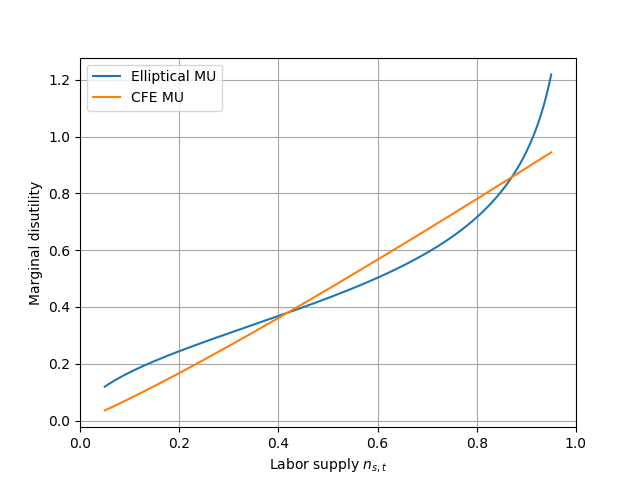
\includegraphics{images/EllipVsCFE_MargUtil.png}}}
  \end{figure}

  \citet{EvansPhillips:2017} propose using an equation for an ellipse to match the disutility of labor supply to whatever traditional functional form one wants. Our preferred specification in \ogindia is to fit an elliptical disutility of labor supply function to approximate a linearly separable constant Frisch elasticity (CFE) functional form. Let $v(n)$ be a general disutility of labor function. A CFE disutility of labor function is the following,
  \begin{equation}\label{EqCFE}
    v(n) \equiv \frac{n^{1+\frac{1}{\theta}}}{1+\frac{1}{\theta}}, \quad\theta > 0
  \end{equation}
  where $\theta>0$ represents the Frisch elasticity of labor supply. The elliptical disutility of labor supply functional form is the following,
  \begin{equation}\label{EqEllipDisut}
    v(n) = -b\left[1 - \left(\frac{n}{\tilde{l}}\right)^\upsilon\right]^{\frac{1}{\upsilon}}, \quad b,\upsilon>0
  \end{equation}
  where $b>0$ is a scale parameter and $\upsilon>0$ is a curvature parameter. This functional form satisfies both $v'(n)>0$ and $v''(n)>0$ for all $n\in(0,1)$. Further, it has Inada conditions at both the upper and lower bounds of labor supply $\lim_{n\rightarrow 0}v'(n) = 0$ and $\lim_{n\rightarrow \tilde{l}}v'(n) = -\infty$.

  Because it is the marginal disutility of labor supply that matters for household decision making, we want to choose the parameters of the elliptical disutility of labor supply function $(b,\upsilon)$ so that the elliptical marginal utilities match the marginal utilities of the CFE disutility of labor supply. Figure \ref{FigMDUcompar} shows the fit of marginal utilities for a Frisch elasticity of $\theta=0.9$ and a total time endowment of $\tilde{l}=1.0$. The estimated elliptical utility parameters in this case are $b=0.527$ and $\upsilon=1.497$.\footnote{\citet{Peterman:2016} shows that in a macro-model that has only an intensive margin of labor supply and no extensive margin and represents a broad composition of individuals supplying labor---such as \ogindia---a Frisch elasticity of around 0.9 is probably appropriate. He tests the implied macro elasticity when the assumed micro elasticities are small on the intensive margin but only macro aggregates---which include both extensive and intensive margin agents---are observed.}


\section{Optimality Conditions}\label{SecHHeulers}

  Households choose lifetime consumption $\{c_{j,s,t+s-1}\}_{s=1}^S$, labor supply $\{n_{j,s,t+s-1}\}_{s=1}^S$, and savings $\{b_{j,s+1,t+s}\}_{s=1}^{S}$ to maximize lifetime utility, subject to the budget constraints and non negativity constraints. The household period utility function is the following.
  \begin{equation}\label{EqHHPerUtil}
    \begin{split}
      u(c_{j,s,t},n_{j,s,t},b_{j,s+1,t+1}) &\equiv \frac{(c_{j,s,t})^{1-\sigma} - 1}{1-\sigma} + e^{g_y t(1-\sigma)}\chi^n_s\biggl(b\left[1 - \left(\frac{n_{j,s,t}}{\tilde{l}}\right)^\upsilon\right]^{\frac{1}{\upsilon}}\biggr) + \\
      &\chi^b_j \rho_s \frac{(b_{j,s+1,t+1})^{1-\sigma} - 1}{1-\sigma} \quad\forall j,t \quad\text{and}\quad E+1 \leq s \leq E+S
    \end{split}
  \end{equation}
  The period utility function \eqref{EqHHPerUtil} is linearly separable in $c_{j,s,t}$, $n_{j,s,t}$, and $b_{j,s+1,t+1}$. The first term is a constant relative risk aversion (CRRA) utility of consumption. The second term is the elliptical disutility of labor described in Section \ref{SecHHellipUtil}. The constant $\chi^n_s$ adjusts the disutility of labor supply relative to consumption and can vary by age $s$, which is helpful for calibrating the model to match labor market moments. See Chapter \ref{Chap_Calibr} for a discussion of the calibration.

  It is necessary to multiply the disutility of labor in \eqref{EqHHPerUtil} by $e^{g_y(1-\sigma)}$ because labor supply $n_{j,s,t}$ is stationary, but both consumption $c_{j,s,t}$ and savings $b_{j,s+1,t+1}$ are growing at the rate of technological progress (see Chapter \ref{Chap_Stnrz}). The $e^{g_y(1-\sigma)}$ term keeps the relative utility values of consumption, labor supply, and savings in the same units.

  The final term in the period utility function \eqref{EqHHPerUtil} is the ``warm glow'' bequest motive. It is a CRRA utility of savings, discounted by the mortality rate $\rho_s$.\footnote{See Section \ref{SecDemogMort} of Chapter \ref{Chap_Demog} for a detailed discussion of mortality rates in \ogindia.} Intuitively, it signifies the utility a household gets in the event that they don't live to the next period with probability $\rho_s$. It is a utility of savings beyond its usual benefit of allowing for more consumption in the next period. This utility of bequests also has constant $\chi^b_j$ which adjusts the utility of bequests relative to consumption and can vary by lifetime income group $j$. This is helpful for calibrating the model to match wealth distribution moments. See Chapter \ref{Chap_Calibr} for a discussion of the calibration. Note that any bequest before age $E+S$ is unintentional as it was bequeathed due an event of death that was uncertain. Intentional bequests are all bequests given in the final period of life in which death is certain $b_{j,E+S+1,t}$.

  The household lifetime optimization problem is to choose consumption $c_{j,s,t}$, labor supply $n_{j,s,t}$, and savings $b_{j,s+1,t+1}$ in every period of life to maximize expected discounted lifetime utility, subject to budget constraints and upper-bound and lower-bound constraints.
  \begin{align}
    &\max_{\{(c_{j,s,t}),(n_{j,s,t}),(b_{j,s+1,t+1})\}_{s=E+1}^{E+S}}\: \sum_{s=1}^S\beta^{s-1}\left[\Pi_{u=E+1}^{E+s}(1 - \rho_u)\right]u(c_{j,s,t+s-1},n_{j,s,t+s-1},b_{j,s+1,t+s}) \label{EqHHmaxprob} \\
    &\quad\text{s.t.}\quad c_{j,s,t} + b_{j,s+1,t+1} = (1 + r_{t})b_{j,s,t} + w_t e_{j,s} n_{j,s,t} + \zeta_{j,s}\frac{BQ_t}{\lambda_j\omega_{s,t}} + \eta_{j,s,t}\frac{TR_{t}}{\lambda_j\omega_{s,t}} - T_{s,t} \tag{\ref{EqHHBC}} \\
    &\qquad\text{and}\quad c_{j,s,t}\geq 0,\: n_{j,s,t} \in[0,\tilde{l}],\:\text{and}\: b_{j,1,t}=0 \quad\forall j, t, \:\text{and}\: E+1\leq s\leq E+S \nonumber
  \end{align}
  The nonnegativity constraint on consumption does not bind in equilibrium because of the Inada condition $\lim_{c\rightarrow 0}u_1(c,n,b') = \infty$, which implies consumption is always strictly positive in equilibrium $c_{j,s,t}>0$ for all $j$, $s$, and $t$. The warm glow bequest motive in \eqref{EqHHPerUtil} also has an Inada condition for savings at zero, so $b_{j,s,t}>0$ for all $j$, $s$, and $t$. This is an implicit borrowing constraint.\footnote{It is important to note that savings also has an implicit upper bound $b_{j,s,t}\leq k$ above which consumption would be negative in current period. However, this upper bound on savings in taken care of by the Inada condition on consumption.} And finally, as discussed in Section \ref{SecHHellipUtil}, the elliptical disutility of labor supply functional form in \eqref{EqHHPerUtil} imposes Inada conditions on both the upper and lower bounds of labor supply such that labor supply is strictly interior in equilibrium $n_{j,s,t}\in(0,\tilde{l})$ for all $j$, $s$, and $t$.

  The household maximization problem can be further reduced by substituting in the household budget constraint, which binds with equality. This simplifies the household's problem to choosing labor supply $n_{j,s,t}$ and savings $b_{j,s+1,t+1}$ every period to maximize lifetime discounted expected utility. The $2S$ first order conditions for every type-$j$ household that characterize the its $S$ optimal labor supply decisions and $S$ optimal savings decisions are the following.

  \begin{equation}\label{EqHHeul_n}
    \begin{split}
      &w_t e_{j,s}\bigl(1 - \tau^{mtrx}_{s,t}\bigr)(c_{j,s,t})^{-\sigma} = e^{g_y(1-\sigma)}\chi^n_{s}\biggl(\frac{b}{\tilde{l}}\biggr)\biggl(\frac{n_{j,s,t}}{\tilde{l}}\biggr)^{\upsilon-1}\Biggl[1 - \biggl(\frac{n_{j,s,t}}{\tilde{l}}\biggr)^\upsilon\Biggr]^{\frac{1-\upsilon}{\upsilon}} \\
      &\qquad\qquad\qquad\qquad\qquad\qquad\qquad\qquad\forall j,t, \quad\text{and}\quad E+1\leq s\leq E+S \\
    \end{split}
  \end{equation}

  \begin{equation}\label{EqHHeul_b}
    \begin{split}
      &(c_{j,s,t})^{-\sigma} = \chi^b_j\rho_s(b_{j,s+1,t+1})^{-\sigma} + \beta\bigl(1 - \rho_s\bigr)\Bigl(1 + r_{t+1}\bigl[1 - \tau^{mtry}_{s+1,t+1}\bigr]\Bigr)(c_{j,s+1,t+1})^{-\sigma} \\
      &\qquad\qquad\qquad\qquad\qquad\qquad\qquad\qquad\forall j,t, \quad\text{and}\quad E+1\leq s\leq E+S-1 \\
    \end{split}
  \end{equation}

  \begin{equation}\label{EqHHeul_bS}
    (c_{j,E+S,t})^{-\sigma} = \chi^b_j(b_{j,E+S+1,t+1})^{-\sigma} \quad\forall j,t \quad\text{and}\quad s = E+S
  \end{equation}



  The distortion of taxation on household decisions can be seen in Euler equations \eqref{EqHHeul_n} and \eqref{EqHHeul_b} in the terms that have a marginal tax rate $(1-\tau^{mtr})$. This comes from the expression for total tax liabilities as a function of the effective tax rate and total income as expressed in \eqref{EqTaxCalcLiabETR}. Using the chain rule, we can break up the derivatives of total tax liability with respect to $n_{j,s,t}$ and $b_{j,s,t}$, respectively, into simpler functions of marginal tax rates. We discuss this in more detail in Chapter \ref{Chap_TaxCalc}.

  \begin{equation}\tag{\ref{EqMTRx_derive}}
    \frac{\partial T_{s,t}}{\partial n_{j,s,t}}  = \frac{\partial T_{s,t}}{\partial w_t e_{j,s}n_{j,s,t}}\frac{\partial w_{t}e_{j,s}n_{j,s,t}}{\partial n_{j,s,t}} = \frac{\partial T_{s,t}}{\partial w_{t}e_{j,s}n_{j,s,t}}w_t e_{j,s} = \tau^{mtrx}_{s,t}w_t e_{j,s}
  \end{equation}

  \begin{equation}\tag{\ref{EqMTRy_derive}}
    \frac{\partial T_{s,t}}{\partial b_{j,s,t}} = \frac{\partial T_{s,t}}{\partial r_{t}b_{j,s,t}}\frac{\partial r_t b_{j,s,t}}{\partial b_{j,s,t}} = \frac{\partial T_{s,t}}{\partial r_t b_{j,s,t}}r_{t} = \tau^{mtry}_{s,t}r_t
  \end{equation}


\section{Expectations}\label{SecHHexp}

  To conclude the household's problem, we must make an assumption about how the age-$s$ household can forecast the time path of interest rates, wages, and total bequests $\{r_u, w_u, BQ_u\}_{u=t}^{t+S-s}$ over his remaining lifetime. As we will show in Chapters \ref{Chap_SSeqlb} and \ref{Chap_NSSeqlb}, the equilibrium interest rate $r_t$, wage $w_t$, and total bequests $BQ_t$ will be functions of the state vector $\bm{\Gamma}_t$, which turns out to be the entire distribution of savings at in period $t$.

  Define $\bm{\Gamma}_t$ as the distribution of household savings across households at time $t$.
  \begin{equation}\label{EqSavDist}
    \bm{\Gamma}_t \equiv \bigl\{b_{j,s,t}\bigr\}_{s=E+2}^{E+S} \quad\forall j,t
  \end{equation}
  Let general beliefs about the future distribution of capital in period $t+u$ be characterized by the operator $\Omega(\cdot)$ such that:
  \begin{equation}\label{EqBeliefs}
    \bm{\Gamma}^e_{t+u} = \Omega^u\left(\bm{\Gamma}_t\right) \quad \forall t, \quad u\geq 1
  \end{equation}
  where the $e$ superscript signifies that $\bm{\Gamma}^e_{t+u}$ is the expected distribution of wealth at time $t+u$ based on general beliefs $\Omega(\cdot)$ that are not constrained to be correct.\footnote{In Chapter \ref{Chap_NSSeqlb} we will assume that beliefs are correct (rational expectations) for the non-steady-state equilibrium in Definition \ref{DefNSSEql}.}
